%!TEX root = ../template.tex
%%%%%%%%%%%%%%%%%%%%%%%%%%%%%%%%%%%%%%%%%%%%%%%%%%%%%%%%%%%%%%%%%%%%
%% chapter4.tex
%% NOVA thesis document file
%%
%% Chapter with lots of dummy text
%%%%%%%%%%%%%%%%%%%%%%%%%%%%%%%%%%%%%%%%%%%%%%%%%%%%%%%%%%%%%%%%%%%%

\typeout{NT FILE chapter4.tex}%

\chapter{Proposal}
\label{cha:proposal}


\begin{figure}[htbp]
    \centering
    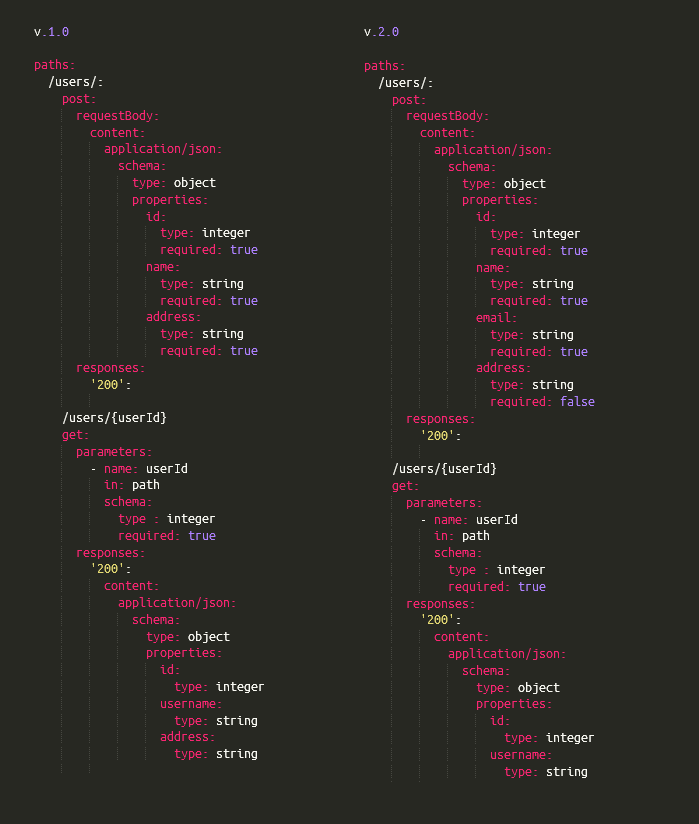
\includegraphics[height=6in]{simple_sig}
    \caption{A Avro schema and its associated serialized record }
    \label{fig:avro}
\end{figure}

Each operation's signature in every contract can be expressed as a function.



The service contracts are written in standard specification language such as OpenAPI;

The versions of service API are collected in a schema registry;

When a new version is submitted for deployment the registry is consulted in order to obtain the set of all active versions of the same service;

For each pair of versions (new, old) a compatibility specification file is produced;



In this file all functions and parameters are associated with a key;

Records are expanded/exploded and each of its parameters is associated with a key, the record itself is also associated with a key;

This file contains the associations between the old version function/parameter keys, and the new version parameters keys (eg. old:k0 -> new:k1; old:k1->new:k5);

This file is audited by a programmer before being used for the generation of the adapter proxy code
In case of incorrect mapping between parameter types the programmer can fix manually.

Some ambiguous evolutions can only be solved with human intervention and knowledge of the domain;
The system notifies the programmer if such a case occurs and request intervention for its resolution.

\begin{figure}[htbp]
    \centering
    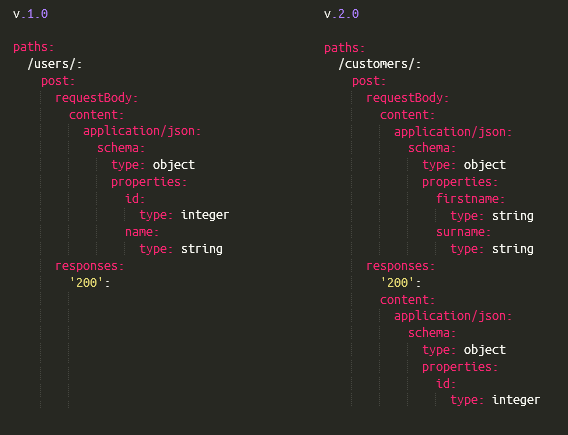
\includegraphics[height=4in]{complez_sig}
    \caption{Complex signature change}
    \label{fig:complex}
\end{figure}

Examples:
renaming two fields of the same type;
inserting a new field and removing another of the same type, is indistinguishable from renaming a field;

Default values can also be supplied inside compatibility specification in order to de-clutter service API or implementations;

More complex signature changes (such as the change of parameter unit from celsius to fahrenheit, the change of date format, the partition of name parameter into surname and first name)
can be accommodated in the combinability specification with the use of functions (eg. extractFirstName(old:k0) -> new:k1  extractSurname(old:k0) -> new:k1)

This functions can be made available through static libraries, or more interestingly, the programmer could write their implementation in the compatibility specification file
and afterwards they would be integrated in adapter proxy coded before compilation;